\clearpage
\section{Efficiencies and systematic uncertainties for simplified models\label{app:signal}}

\subsection{T2cc\label{app:t2cc}}

%\begin{figure}[h!]
%  \begin{center}
%    \subfigure[$m_{\sTop} = 250\gev, m_{\rm LSP} = 170\gev$]{
%      \includegraphics[width=0.6\textwidth, trim=0 0 0 30, clip=true]{figures/sms/t2cc/v25/T2cc_sig_inj_250_170}
%    } \\
%%    \subfigure[$m_{\sTop} = 250\gev, m_{\rm LSP} = 230\gev$]{
%%      \includegraphics[width=0.6\textwidth, trim=0 0 0 30, clip=true]{figures/sms/t2cc/v25/T2cc_sig_inj_250_230}
%%    } \\
%    \subfigure[$m_{\sTop} = 250\gev, m_{\rm LSP} = 240\gev$]{
%      \includegraphics[width=0.6\textwidth, trim=0 0 0 30, clip=true]{figures/sms/t2cc/v25/T2cc_sig_inj_250_240}
%    } \\
%    \caption{The expected signal significance (in terms of the number
%      of standard deviations) per signal region bin for the
%      \texttt{T2cc} model with $m_{\sTop} = 250\gev$ and $m_{\rm LSP}
%      = 170\gev$ (Top) and $m_{\rm LSP} = 170\gev$ (Bottom).}
%    % the best fit point $m_{\rm LSP} = 170\gev$ (Middle) 
%    \label{fig:sms-t2cc-sig}
%  \end{center}
%\end{figure}

\begin{figure}[h!]
  \begin{center}
    \subfigure[\label{fig:sms-pdf-t2cc-0b_le3j}\njetlow, $\nb = 0$]{
      \includegraphics[width=0.43\textwidth,page=2]{figures/sms/t2cc/v1/t2cc_unc}
    }
    \subfigure[\label{fig:sms-pdf-t2cc-1b_le3j}\njetlow, $\nb = 1$]{
      \includegraphics[width=0.43\textwidth,page=2]{figures/sms/t2cc/v1/t2cc_unc}
    }\\
    \subfigure[\label{fig:sms-pdf-t2cc-0b_ge4j}\njethigh, $\nb = 0$]{
      \includegraphics[width=0.43\textwidth,page=2]{figures/sms/t2cc/v1/t2cc_unc}
    }
    \subfigure[\label{fig:sms-pdf-t2cc-1b_ge4j}\njethigh, $\nb = 1$]{
      \includegraphics[width=0.43\textwidth,page=2]{figures/sms/t2cc/v1/t2cc_unc}
    }\\
    \caption{\label{fig:sms-pdf-t2cc}Ratio of efficiency times
      acceptance for the (middle) central value, (top) $+1\sigma$
      value, (bottom) $-1\sigma$ value of the envelope calculation
      relative to the nominal PDF set used to produce the
      \texttt{T2cc} sample. }
  \end{center}
\end{figure}

\begin{figure}[h!]
  \begin{center}
    \subfigure[\njetlow, $\nb = 0$.]{
      \includegraphics[width=0.35\textwidth, page=7]{figures/sms/t2cc/v1/t2cc_unc}
    }
    \subfigure[\njetlow, $\nb = 0$.]{
      \includegraphics[width=0.35\textwidth, page=6]{figures/sms/t2cc/v1/t2cc_unc}
    }\\
    \subfigure[\njetlow, $\nb = 1$.]{
      \includegraphics[width=0.35\textwidth, page=14]{figures/sms/t2cc/v1/t2cc_unc}
    }
    \subfigure[\njetlow, $\nb = 1$.]{
      \includegraphics[width=0.35\textwidth, page=13]{figures/sms/t2cc/v1/t2cc_unc}
    }\\
    \subfigure[\njethigh, $\nb = 0$.]{
      \includegraphics[width=0.35\textwidth, page=28]{figures/sms/t2cc/v1/t2cc_unc}
    }
    \subfigure[\njethigh, $\nb = 0$.]{
      \includegraphics[width=0.35\textwidth, page=27]{figures/sms/t2cc/v1/t2cc_unc}
    }\\
    \subfigure[\njethigh, $\nb = 1$.]{
      \includegraphics[width=0.35\textwidth, page=35]{figures/sms/t2cc/v1/t2cc_unc}
    }  
    \subfigure[\njethigh, $\nb = 1$.]{
      \includegraphics[width=0.35\textwidth, page=34]{figures/sms/t2cc/v1/t2cc_unc}
    }\\
    \caption{\label{fig:sms-jes-t2cc}The fractional change in
      signal efficiency due to systematically (Left) increasing and
      (Middle) decreasing all jet energies, and (Right) the resulting
      (symmetric) systematic uncertainties due to JES uncertainties
      for \texttt{T2cc}.}
  \end{center}
\end{figure}

\begin{figure}[h!]
  \begin{center}
    \subfigure[\njetlow, $\nb = 0$.]{
      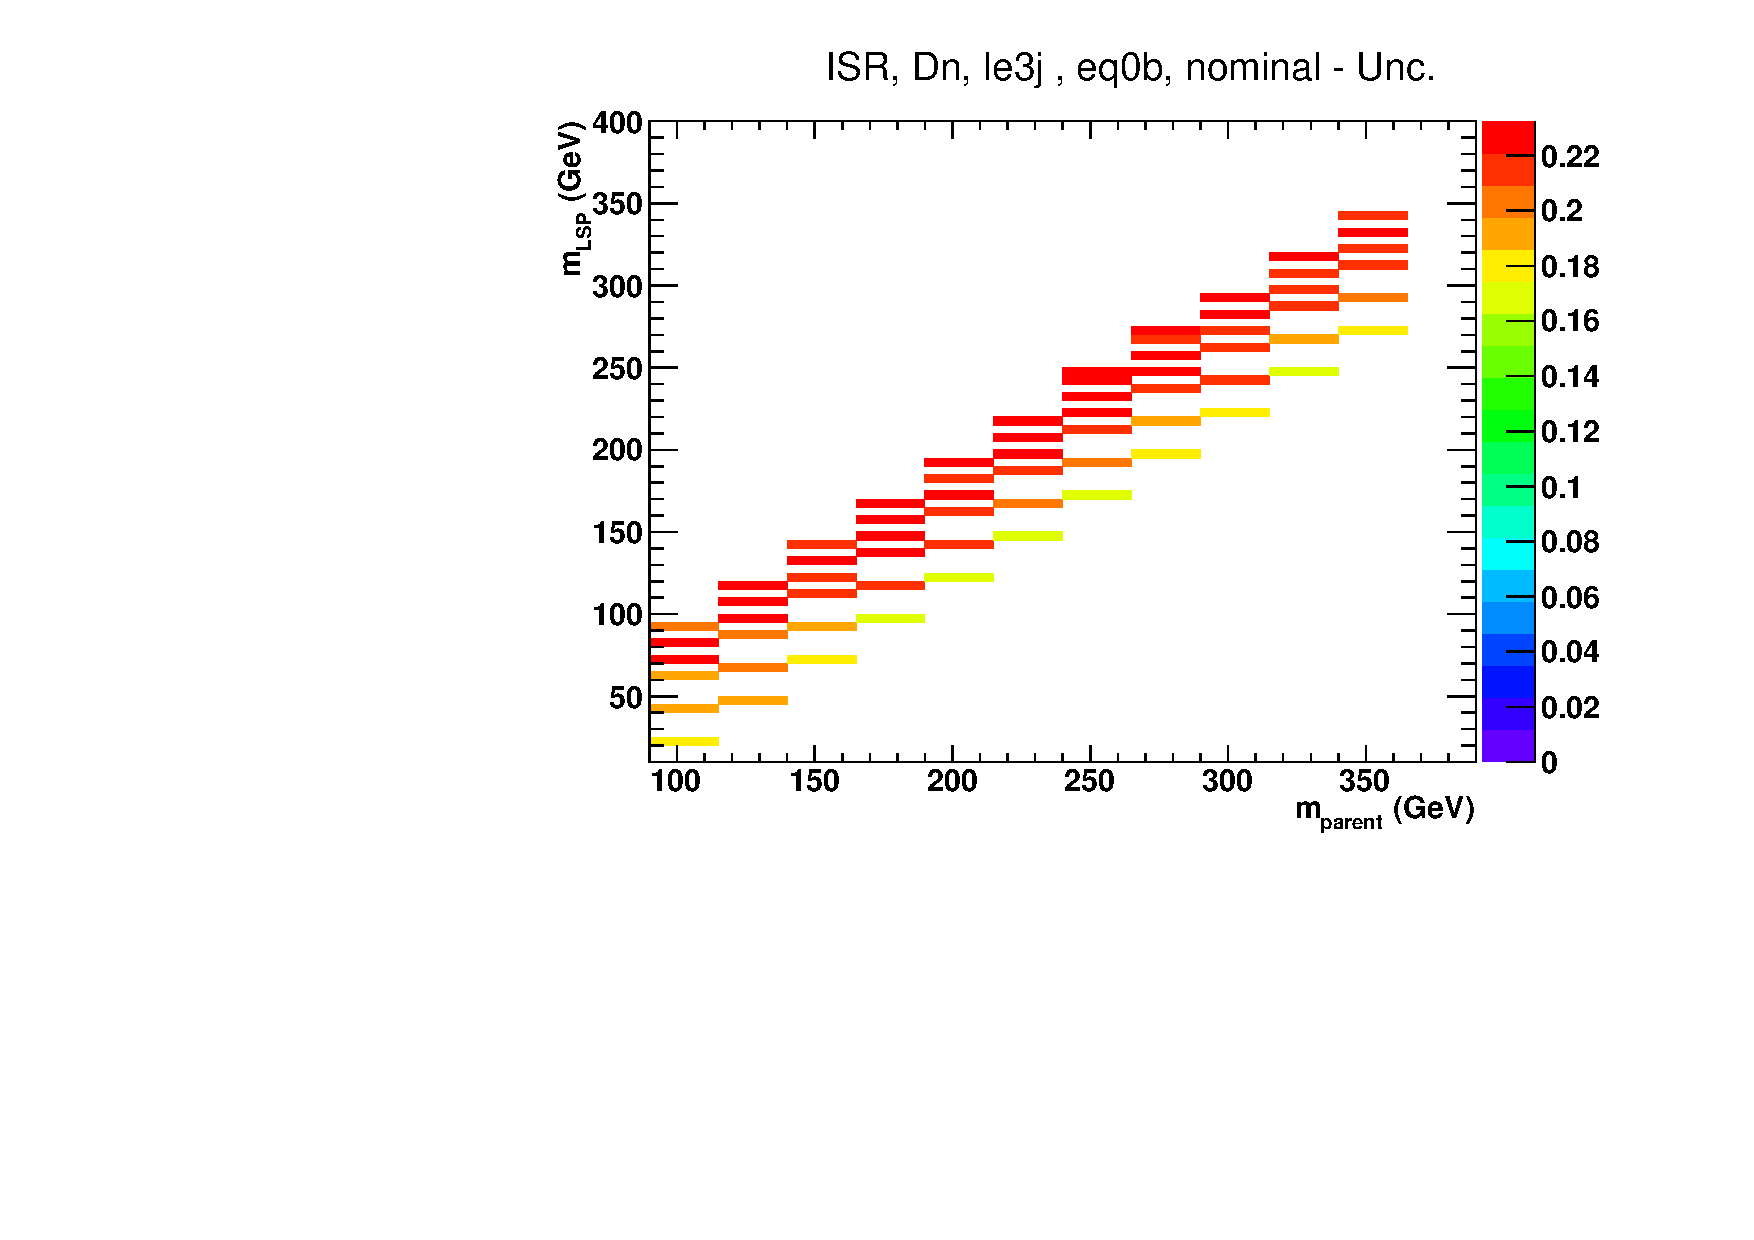
\includegraphics[width=0.35\textwidth, page=1]{figures/sms/t2cc/v1/t2cc_unc}
    }
    \subfigure[\njetlow, $\nb = 0$.]{
      \includegraphics[width=0.35\textwidth, page=4]{figures/sms/t2cc/v1/t2cc_unc}
    }\\
    \subfigure[\njetlow, $\nb = 1$.]{
      \includegraphics[width=0.35\textwidth, page=8]{figures/sms/t2cc/v1/t2cc_unc}
    }
    \subfigure[\njetlow, $\nb = 1$.]{
      \includegraphics[width=0.35\textwidth, page=11]{figures/sms/t2cc/v1/t2cc_unc}
    }\\
    \subfigure[\njethigh, $\nb = 0$.]{
      \includegraphics[width=0.35\textwidth, page=22]{figures/sms/t2cc/v1/t2cc_unc}
    }
    \subfigure[\njethigh, $\nb = 0$.]{
      \includegraphics[width=0.35\textwidth, page=25]{figures/sms/t2cc/v1/t2cc_unc}
    }\\
    \subfigure[\njethigh, $\nb = 1$.]{
      \includegraphics[width=0.35\textwidth, page=29]{figures/sms/t2cc/v1/t2cc_unc}
    }  
    \subfigure[\njethigh, $\nb = 1$.]{
      \includegraphics[width=0.35\textwidth, page=32]{figures/sms/t2cc/v1/t2cc_unc}
    }\\
    \caption{\label{fig:sms-isr-t2cc}The fractional change in signal
      efficiency due to systematically (Left) increasing and (Middle)
      decreasing event weights according to ISR uncertainties, and
      (Right) the resulting (symmetric) systematic uncertainties due
      to ISR uncertainties for \texttt{T2cc}.}
  \end{center}
\end{figure}

\begin{figure}[h!]
  \begin{center}
    \subfigure[\njetlow, $\nb = 0$.]{
      \includegraphics[width=0.35\textwidth, page=3]{figures/sms/t2cc/v1/t2cc_unc}
    }
    \subfigure[\njetlow, $\nb = 0$.]{
      \includegraphics[width=0.35\textwidth, page=5]{figures/sms/t2cc/v1/t2cc_unc}
    }\\
    \subfigure[\njetlow, $\nb = 1$.]{
      \includegraphics[width=0.35\textwidth, page=10]{figures/sms/t2cc/v1/t2cc_unc}
    }
    \subfigure[\njetlow, $\nb = 1$.]{
      \includegraphics[width=0.35\textwidth, page=12]{figures/sms/t2cc/v1/t2cc_unc}
    }\\
    \subfigure[\njethigh, $\nb = 0$.]{
      \includegraphics[width=0.35\textwidth, page=24]{figures/sms/t2cc/v1/t2cc_unc}
    }
    \subfigure[\njethigh, $\nb = 0$.]{
      \includegraphics[width=0.35\textwidth, page=26]{figures/sms/t2cc/v1/t2cc_unc}
    }\\
    \subfigure[\njethigh, $\nb = 1$.]{
      \includegraphics[width=0.35\textwidth, page=31]{figures/sms/t2cc/v1/t2cc_unc}
    }  
    \subfigure[\njethigh, $\nb = 1$.]{
      \includegraphics[width=0.35\textwidth, page=33]{figures/sms/t2cc/v1/t2cc_unc}
    }\\
    \caption{\label{fig:sms-btag-t2cc}The fractional change in signal
      efficiency due to systematically (Left) increasing and (Middle)
      decreasing all b-tag efficiencies according to the scale factor
      uncertainties, and (Right) the resulting (symmetric) systematic
      uncertainties due to b-tag scale factor uncertainties for
      \texttt{T2cc}.} 
  \end{center}
\end{figure}

\begin{figure}[h!]
  \begin{center}
    \subfigure[\njetlow, $\nb = 0$.]{
     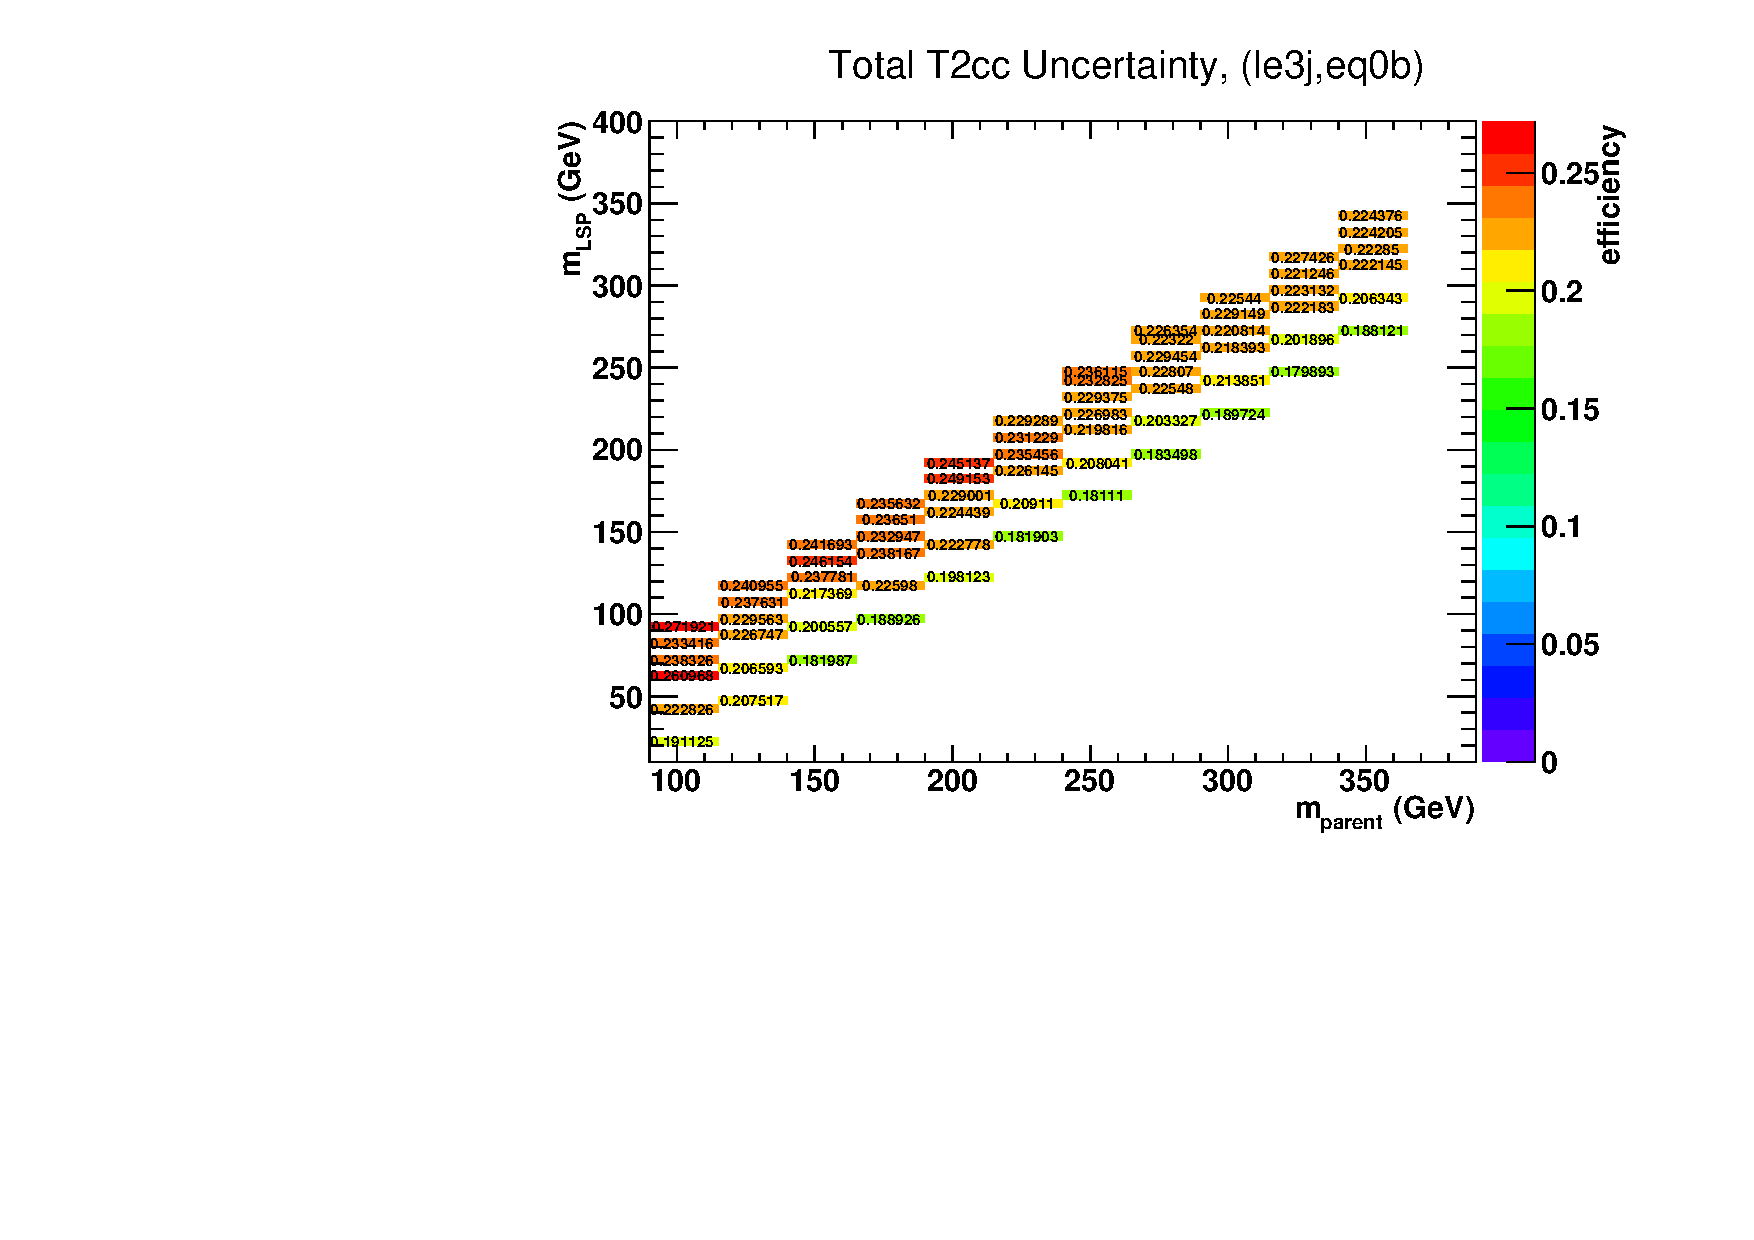
\includegraphics[width=0.48\textwidth,page=1]{figures/sms/t2cc/v1/t2cc_pfJet_totalUnc.pdf}
    }                                                                  
    \subfigure[\njetlow, $\nb = 1$.]{                                  
     \includegraphics[width=0.48\textwidth,page=2]{figures/sms/t2cc/v1/t2cc_pfJet_totalUnc.pdf}
    }\\                                                                
    \subfigure[\njethigh, $\nb = 0$.]{                                 
      \includegraphics[width=0.48\textwidth,page=5]{figures/sms/t2cc/v1/t2cc_pfJet_totalUnc.pdf}
    }                                                                  
    \subfigure[\njethigh, $\nb = 1$.]{                                 
      \includegraphics[width=0.48\textwidth,page=6]{figures/sms/t2cc/v1/t2cc_pfJet_totalUnc.pdf}
    }\\
    \caption{\label{fig:sms-total-t2cc}The total systematic
      uncertainty in the signal efficiency times acceptance for all
      relevant event categories for the \texttt{T2cc} intepretation.}
  \end{center}
\end{figure}

%\FloatBarrier
%%%%%%%%%%%%%%%%%%%%%%%%%%%%%%%%%%%%%%%%%%%%%%%%%%%%%%%%%%%%%%%%%%%%%%%%%%%%%%%%
%%%%%%%%%%%%%%%%%%%%%%%%%%%%%%%%%%%%%%%%%%%%%%%%%%%%%%%%%%%%%%%%%%%%%%%%%%%%%%%%
%%%%%%%%%%%%%%%%%%%%%%%%%%%%%%%%%%%%%%%%%%%%%%%%%%%%%%%%%%%%%%%%%%%%%%%%%%%%%%%%

\clearpage
\subsection{T2tt\label{app:t2tt}}


%\begin{figure}[!h]
%  \begin{center}
%    \subfigure[Hadronic Selection Efficiency, (2--3,1)]{
%      \includegraphics[width=0.4\textwidth,page=7]{figures/sms/t2tt/v1/T2tt_eff}
%    } 
%    \subfigure[Hadronic Selection Efficiency, (2--3,2)]{
%      \includegraphics[width=0.4\textwidth,page=8]{figures/sms/t2tt/v1/T2tt_eff}
%    } \\
%%    \subfigure[Hadronic Selection Efficiency, ($\geq 4$,0)]{
%%      \includegraphics[width=0.4\textwidth]{figures/sms/t2_4body/v6/T2_4body_had_eff_maps_eq0b_ge4j_SITV}
%%    }     
%%    \subfigure[Hadronic Selection Efficiency, ($\geq 4$,1)]{
%%      \includegraphics[width=0.4\textwidth]{figures/sms/t2_4body/v6/T2_4body_had_eff_maps_eq1b_ge4j_SITV}
%%    } \\
%    \caption{Hadronic selection efficiency times acceptance for the \texttt{T2tt}
%      for the relevant event categories defined by \njet and \nb.
%       Note the different z-axis scales.}
%    \label{fig:sms-eff-t2_4body}
%  \end{center}
%\end{figure}
%
\begin{figure}[h!]
  \begin{center}
    \subfigure[\label{fig:sms-pdf-t2tt-1b_le3j}\njetlow, $\nb = 1$]{
      \includegraphics[width=0.43\textwidth,page=2]{figures/sms/t2tt/v1/t2tt_unc}
    }
    \subfigure[\label{fig:sms-pdf-t2tt-2b_le3j}\njetlow, $\nb = 2$]{
      \includegraphics[width=0.43\textwidth,page=2]{figures/sms/t2tt/v1/t2tt_unc}
    }\\
    \caption{\label{fig:sms-pdf-t2tt}Ratio of efficiency times
      acceptance for the (middle) central value, (top) $+1\sigma$
      value, (bottom) $-1\sigma$ value of the envelope calculation
      relative to the nominal PDF set used to produce the
      \texttt{T2tt} sample. }
  \end{center}
\end{figure}

\begin{figure}[h!]
  \begin{center}
    \subfigure[\njetlow, $\nb = 1$.]{
      \includegraphics[width=0.35\textwidth, page=14]{figures/sms/t2tt/v1/t2tt_unc}
    }
    \subfigure[\njetlow, $\nb = 1$.]{
      \includegraphics[width=0.35\textwidth, page=13]{figures/sms/t2tt/v1/t2tt_unc}
    }\\
    \subfigure[\njetlow, $\nb = 2$.]{
      \includegraphics[width=0.35\textwidth, page=21]{figures/sms/t2tt/v1/t2tt_unc}
    }
    \subfigure[\njetlow, $\nb = 2$.]{
      \includegraphics[width=0.35\textwidth, page=20]{figures/sms/t2tt/v1/t2tt_unc}
    }\\
    \caption{\label{fig:sms-jes-t2tt}The fractional change in
      signal efficiency due to systematically (Left) increasing and
      (Middle) decreasing all jet energies, and (Right) the resulting
      (symmetric) systematic uncertainties due to JES uncertainties
      for \texttt{T2tt}.}
  \end{center}
\end{figure}

\begin{figure}[h!]
  \begin{center}
    \subfigure[\njetlow, $\nb = 1$.]{
      \includegraphics[width=0.35\textwidth, page=8]{figures/sms/t2tt/v1/t2tt_unc}
    }
    \subfigure[\njetlow, $\nb = 1$.]{
      \includegraphics[width=0.35\textwidth, page=11]{figures/sms/t2tt/v1/t2tt_unc}
    }\\
    \subfigure[\njetlow, $\nb = 2$.]{
      \includegraphics[width=0.35\textwidth, page=15]{figures/sms/t2tt/v1/t2tt_unc}
    }
    \subfigure[\njetlow, $\nb = 2$.]{
      \includegraphics[width=0.35\textwidth, page=18]{figures/sms/t2tt/v1/t2tt_unc}
    }\\
    \caption{\label{fig:sms-isr-t2tt}The fractional change in signal
      efficiency due to systematically (Left) increasing and (Middle)
      decreasing event weights according to ISR uncertainties, and
      (Right) the resulting (symmetric) systematic uncertainties due
      to ISR uncertainties for \texttt{T2tt}.}
  \end{center}
\end{figure}

\begin{figure}[h!]
  \begin{center}
    \subfigure[\njetlow, $\nb = 1$.]{
      \includegraphics[width=0.35\textwidth, page=10]{figures/sms/t2tt/v1/t2tt_unc}
    }
    \subfigure[\njetlow, $\nb = 1$.]{
      \includegraphics[width=0.35\textwidth, page=12]{figures/sms/t2tt/v1/t2tt_unc}
    }\\
    \subfigure[\njetlow, $\nb = 2$.]{
      \includegraphics[width=0.35\textwidth, page=17]{figures/sms/t2tt/v1/t2tt_unc}
    }
    \subfigure[\njetlow, $\nb = 2$.]{
      \includegraphics[width=0.35\textwidth, page=19]{figures/sms/t2tt/v1/t2tt_unc}
    }\\
    \caption{\label{fig:sms-btag-t2tt}The fractional change in signal
      efficiency due to systematically (Left) increasing and (Middle)
      decreasing all b-tag efficiencies according to the scale factor
      uncertainties, and (Right) the resulting (symmetric) systematic
      uncertainties due to b-tag scale factor uncertainties for
      \texttt{T2tt}.} 
  \end{center}
\end{figure}


\begin{figure}[h!]
  \begin{center}
    \subfigure[\njetlow, $\nb = 1$.]{
     \includegraphics[width=0.48\textwidth,page=2]{figures/sms/t2tt/v1/t2tt_pfJet_totalUnc.pdf}
    }
    \subfigure[\njetlow, $\nb = 2$.]{
     \includegraphics[width=0.48\textwidth,page=3]{figures/sms/t2tt/v1/t2tt_pfJet_totalUnc.pdf}
    }\\       
    \caption{\label{fig:sms-total-t2tt}The total systematic
      uncertainty in the signal efficiency times acceptance for all
      relevant event categories for the \texttt{T2tt} intepretation.}
  \end{center}
\end{figure}

